\section{Durchführung}
\label{sec:Durchführung}
\paragraph{verwendete Geräte}
Als Heizelement wird ein Peltier-Element verwendet. Da es abhängig von der Polung der Betriebsspannung eine Seite heizt und die andere kühlt eignet es sich besonders gut für die dynamische Messung über Wärmewellen. Die Erfassung der Daten erfolgt über ein Temperatur Array mit dem daran angeschlossenen \textit{Xplorer GLX}. Dieses Gerät übernimmt alle digitale Verarbeitung.
\begin{figure}
  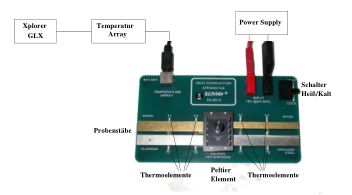
\includegraphics{./logos/Aufbau.PNG}
  \caption{Aufbau zur Messung der Wärmeleitfähigkeit von Metallen. \cite{Anleitung}}
  \label{fig:Aufbau}
\end{figure}
\paragraph{Statische Methode}
Bei der Statischen Messung der Wärmeleitfähigkeit werden die zu untersuchenden Stäber mit einer konstanten Temperatur geheizt und an zwei Stellen der Stäbe (eine nah am Heizelement, eines weiter entfernt) die Temperatur gemessen. Die Verläufe dieser gemessenen Temperaturen werden aufgezeichnet. Hierraus lässt sich die Wärmeleitfähigkeit bestimmen. Die Betriebsspannung wird auf $7\si{\volt}$ eingestellt, die Abtastrate am Xplorer auf $5\si{\second}$.
\paragraph{Dynamische Methode}
Bei der dynamischen Messung der Wärmeleitfähigkeit werden die Stäbe einmal abwechselnd für 40s geheizt und gekühlt, das zweite Mal werden 100s lang geheizt und gekühlt. Die Betriebsspannung wird auf $10\si{\volt}$, die Abtastrate auf $2 \si{\second}$ eingestellt.
